\documentclass{article}
\usepackage[utf8]{inputenc}

\title{Lecture 10: classfication}
\author{wbg231 }
\date{November 2022}
\usepackage{tikz,graphicx,amsmath,amsfonts,amscd,amssymb,bm,cite,epsfig,epsf,url}
\begin{document}

\maketitle

\section{introduction}
\subsection{how to think about it }
\begin{itemize}
%\item 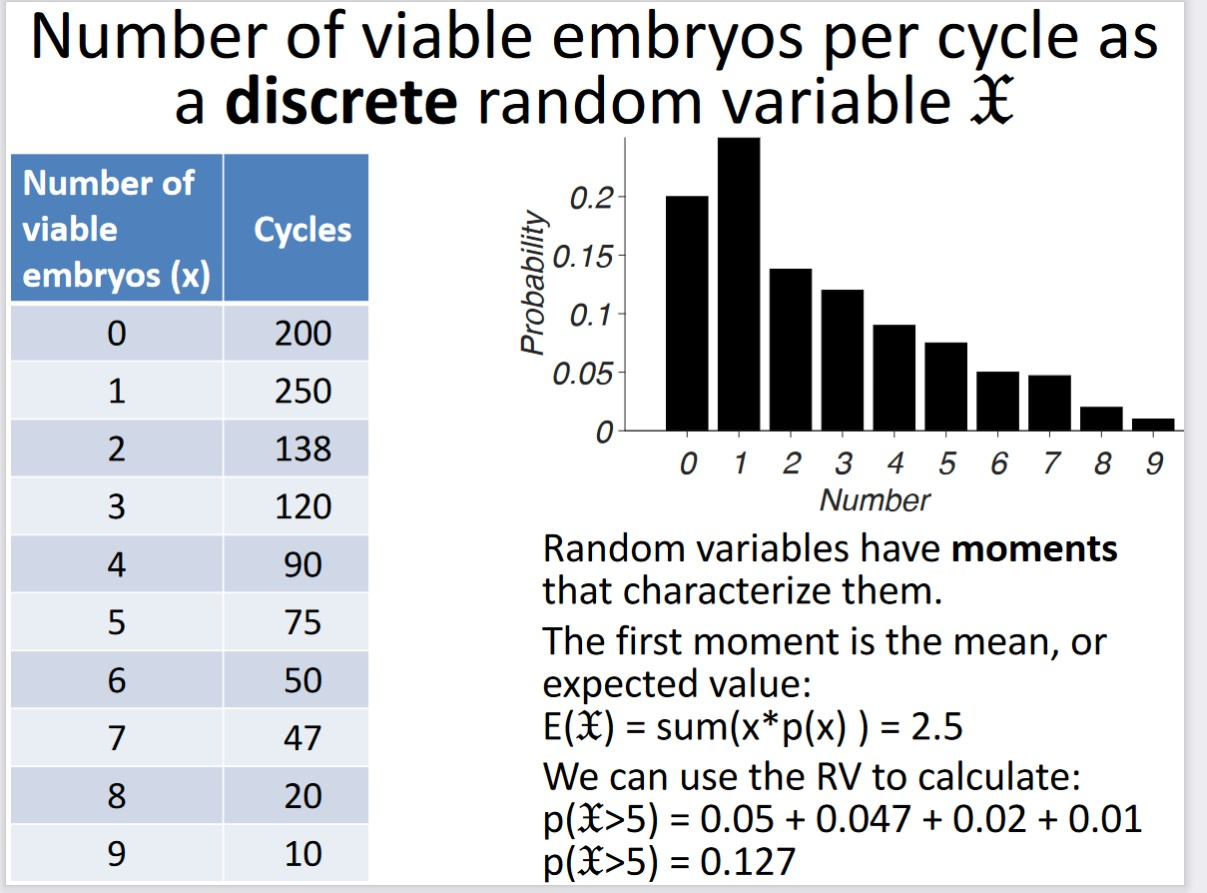
\includegraphics[width=7.5cm]{Final_Review/Lecture_2/lecture_1example.jpg}
\item we are dealing with supervised models
\item we are given a data set X which has individuals and our goal is to categorize each individual in the data set
\item everything we are dealing with today has only two classes. 
\subsection{prediction to classification}
\item in prediction the goal is to find a line that minimizes the distance from our predictions to the actual outcomes 
\item classification, we want to find a hyper plane (this is 1 less than the number of dimensions we are working with), that linearly separates two classes 
\item these problems are inverses, one we are getting as close as possible one we are getting as far as possible 
\section{Logistic Regression}
\subsection{introduction}
\item logistic regression is a bridge from linear regression to classification. this is the most common ml algo likely
\item logistic regression is good because it is fast, and it yields a probability of an individual being in a certain class. 
\item takes continuous inputs and outputs discrete values
\item mapping continuous inputs to binary outcomes while using non-linear linking functions
\item the running example is classifying will you get the degree or not
\item another big example is medical diagnosis
\subsection{example}
\item given your input will you get a job or not 
\item you either get a job or you do not, is that a 50\% chance, no that is a naive fallacy.
\item so we are just looking at gpa and if you get a job. 
\item there is no clear cut off, some people get a job with a low gpa, some have a high gpa did not get the job.
\item suppose the scatter plot looks like this 
\item 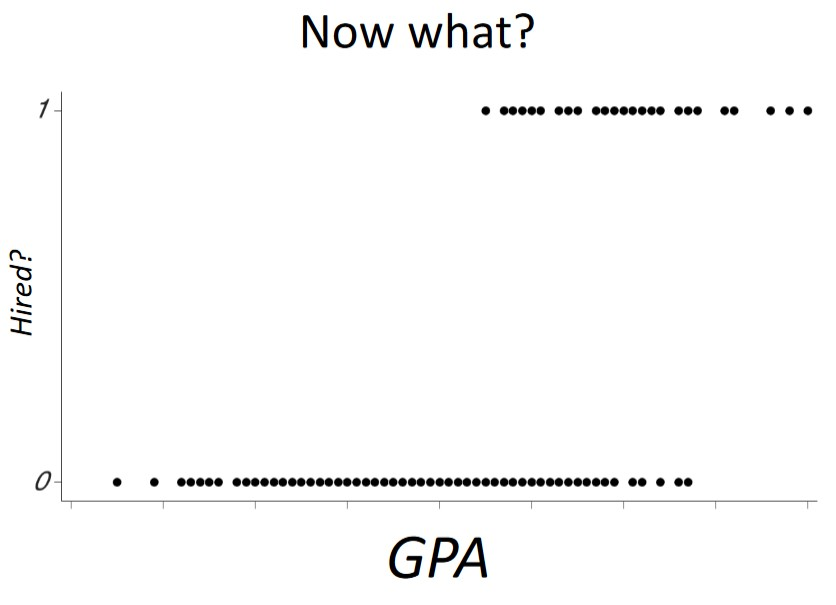
\includegraphics[width=5cm]{Final_Review/lecture_10/logistic_reg.jpg}
\item you can fit a linear regression to this data, but that does not make sense for three reasons 
\begin{enumerate}
    \item it assumes a constant relationship there is a range where a small change in a gpa makes no point, and a range where a small gpa change makes a large change 
    linear regression is unbound 
    \item there are no outcomes except for being hired or not, there is nothing beyond getting hired  or not 
    \item the data is not distributed normally which does not make sense

    
\end{enumerate}
\item it is pretty common to try to fit a linear regression to something that is classification 
\item the logistic regression was designed to fix these issues. 
\subsection{logistic regression}
\item provides a non linear model that links predictors and the outcome 
\item they give odds of something happening which are$odds=\frac{P(p)}{P(p^c)}=\frac{p}{1-p}$
\subsection{logit function }
\item links the value in the predictor viable to the probabilities of the outcomes.
\item we need to estimate this form data 
\item logit is the natural log of the odds.
\item $logit(p)=ln(ods)=ln(\frac{p}{1-p)})=\beta_0+\beta_1 x_1$
\item where the $\beta$ are our parameters and x is our data 
\item here is what the logistic function looks like
\item 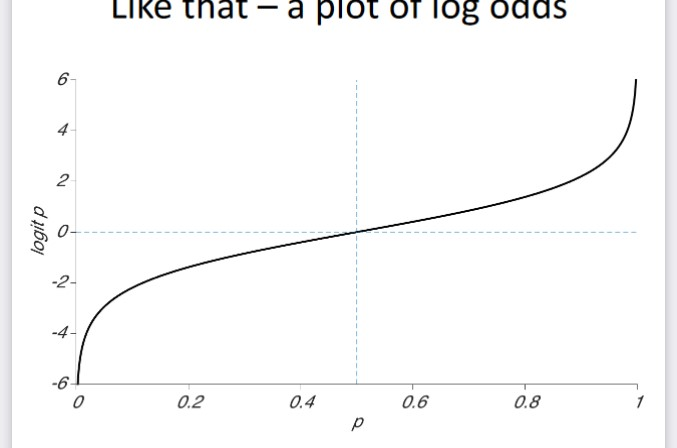
\includegraphics[width=5cm]{Final_Review/lecture_10/logit.jpg}
\item we like a few things about the logit 
\begin{enumerate}
    \item the impact of an x unit change is changing 
    \item it is bounded 
\end{enumerate}
\item so that is 2 out of 3 
\item the issue is this function takes probability as an input and logit as an output
\item so we need to invert it to get what we want 
\item $logit^{-1}(x)=\frac{e^x}{1+e^x}$ this is the inverted logit function 
\item $logit(p)=ln(ods)=ln(\frac{p}{1-p)})=\beta_0+\beta_1 x_1$ then we see that $\frac{p}{1-p}=e^{b_0+\beta_1 x}$ which we can solve as $p=\frac{e^{b_0+\beta_1 x}}{1+e^{b_0+\beta_1 x}}$ (this is the sigmoid function also called the logistic function)
\item it looks like this 
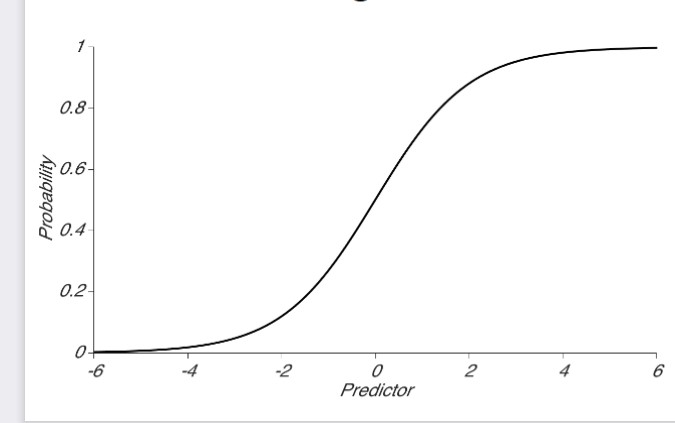
\includegraphics[width=5cm]{Final_Review/lecture_10/sigmoid.jpg}
\item this has good properties
\begin{enumerate}
    \item the outcome is the outcome of probability
    \item it is bounded between 0 and 1 
    \item the impact of the unit change is not equal
\end{enumerate}
\item so this solved all the things we were looking for 
\item then we estimate $\beta$ using maximum likelihood estimation 
\subsection{impact of changing $\beta$}
\item $\beta_0$ is our interpret $\beta_1$ is our slope
\item as $\beta_0$ goes up the function is shifted to the lifted, and thus the location of the inflection point (the point where probability is .5)
\item what is our $\beta_1$ increases our curve gets more steep
\item if $\beta_1$ is infinite it is just a hard cut off 
\subsection{logistic classification}
\item the sigmoid function outputs a probability so we set a threshold where depending on if the value is about or bellow the threshold we output a class

\section{assessment metrics}
\item we want something similar to $r^2$ for regression models
\item a good starting point is accuracy,  that is the number of times we predict correctly over the total number of cases but this does not tell us a lot if there is imbalance in our categories. for instance if 99\% of transactions are not fraud and our model always predicts something is not fraud it will be 99\% accurate
\item we need to think of the different types of errors that can be made
\item the most common one is the AUC area under the ROC curve also called AUROC
\subsection{confusion matrix}
\item this comes to us form medicine and we are going to use that example
\item ROC can be derived from the confusion matrix 
\item 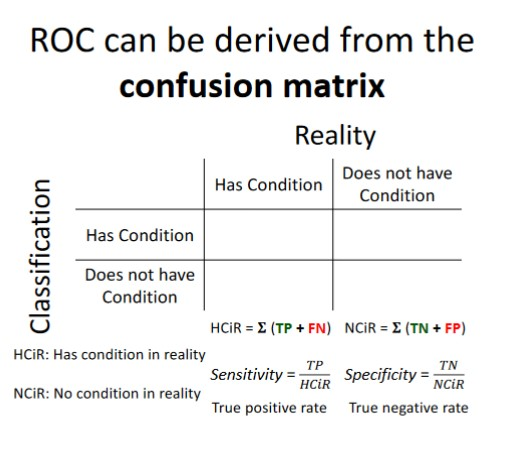
\includegraphics[width=5cm]{Final_Review/lecture_10/confusion_matix_class.jpg}
\item cell 1 is true positives 
\itme cell 2 is false positive 
\item cell 3 is false negative 
\item cell 4 is true negative
\item sensitivity$\frac{tp}{TP+FN}$ ie how how sensitive was our model at picking up that someone has the condition 
\item this started in radar operators, in 1945 it was a big question
\item Specificity$\frac{tn}{tn+fp}$
\item we want a number that integrates all of this information 
\subsection{ROC derivation}
\item the signal distribution is the distribution if our predictor y if there is a condition present 
\item the null distribution is the distribution of our predictor variable y if the condition is not present
\item 
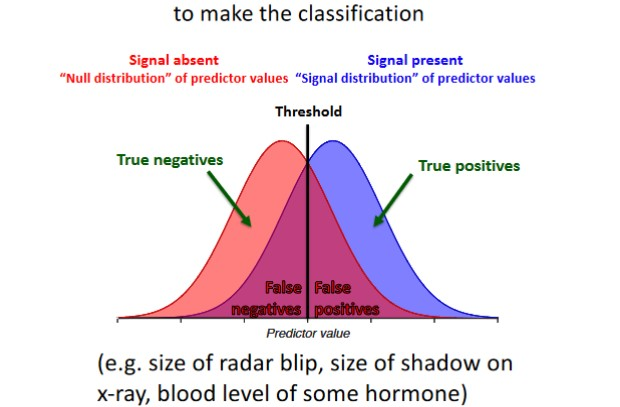
\includegraphics[width=10cm]{Final_Review/lecture_10/null_and_signal.jpg}
\item the red curve is our null distribution (ie y if condition c is 0)
\item the blue curve is our signal distribution (ie y if condition c is 1)
\item we can set our threshold, the value at which if the model's predicted value of y is above that it predicts class c=1 ,and otherwise class c=0
\item but this yields 4 cases
\begin{enumerate}
    \item the part just in the blue curve and to the right of the threshold are true positives, we say they come from the sing la and they did 
    \item the part just in right are true negatives as they are just in the red and to the left of the threshold
    \item the part of the red graph that are beyond the threshold are false positives
    \item the part of the blue graph that are bellow the the threshold are false negatives
\end{enumerate}
\item the only fulcrum we have in this is where to set the threshold
\item moving the threshold to the right will give you fewer true positives, but also less false positives 
\item if you move the threshold to the left you will get fewer true negatives but more false positives
\item we want a number that integrates this 
\subsection{ROC }
\item plotting the sensitivity (true positive rate) as a function of the false positive rate (1-specificity) as we sweet the threshold form all the way to the left to all the way to right 
\item Roc curve name comes from the fact that different radar receiver operators have different personal thresholds for what they call a bird or a plain 
\item 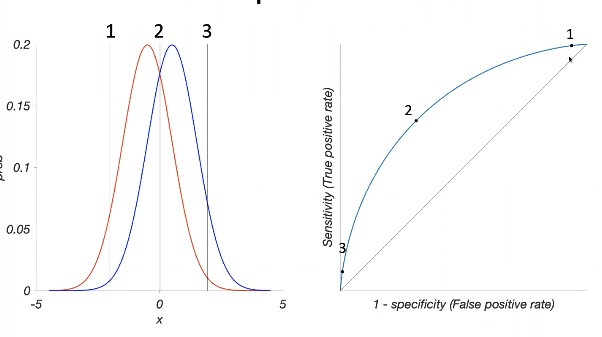
\includegraphics[width=10cm]{Final_Review/lecture_10/roc example.jpg}
\item the gray line is what we would get if we were randomly guessing it is .5, ie the area under the curve is .5
\item if the area under the roc curve is less than .5 then it is worse than random chance. 
\item no matter where you set the threshold, you will be on the roc curve. 
\item so the goal is to get a very l shaped or steep curve.
\item if we want to decrease false positives we can raise our threshold, that is make it more rare for something to be classified as a positive class pushing us towards point 3 but we will have more true positives.
\item for a really bad classifier it does not matter where we set the threshold it is bad any where
\item for a really good classifier we likely want to take point 2, since that would balance
\item once a classifier is set we can not get off this curve. 
\item the AUC is the area under that left curve. 
\item this is used everywhere that classification is used.
\subsection{how good is logistic regression}
\item it works pretty well in terms of roc curve 
\item it is quick 
\item it is understandable 
\item the auc is a single number of 0.5, 1

\item 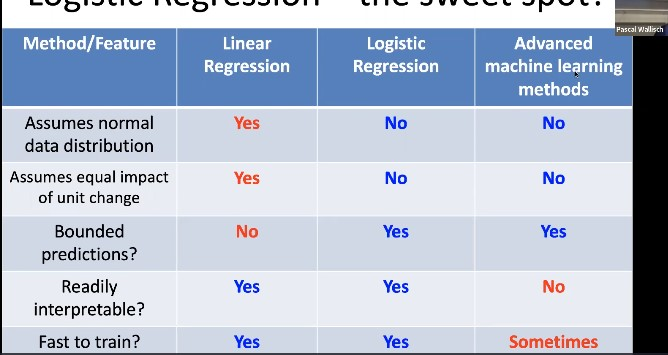
\includegraphics[width=10cm]{Final_Review/lecture_10/trade_off_logistic_reg.jpg}
\item logistic regression is pretty good, it does not over fit much. it trains fast is interpretive does not have  lot of assumptions 
\section{Support Vector Machines}
\subsection{introduction}
\item sounds intimidating is not really, we are just looking for a hyper plane that maximal separates two classes.
\item in linear regression the outliers are the most impact full to the slope of the line 
\itme in SVM only a few points matter at all in defining the hyper plane 
\subsection{example}
\item depression diagnostic is our task 
\item we ware going to pass a linear separable hyperplane that classifies the two groups as well as possible. 
\item if we take our threshold to be to close to out classes, then a new data point that may be closer to a different class than how they are classified 
\item the maximal marginal classifier maximises the distance between the two edges ie the two closest together points of different classifiers
\item 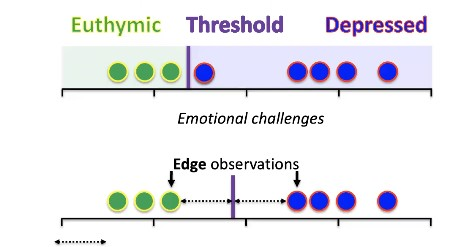
\includegraphics[width=10cm]{Final_Review/lecture_10/margin_class.jpg}
\item so where we put the margin matter's
\subsection{extend this example to 2d}
\item 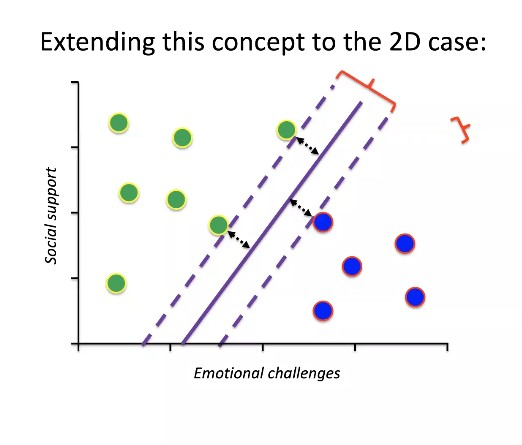
\includegraphics[width=10cm]{Final_Review/lecture_10/2dmargin.jpg}

\item we have emotional challenges and social support as predictors of depression 
\item to be linearly separable we have to be able to draw a line that cuts the two groups with out any overlap
\item the three points that touch the margin are the support vector they define the whole hyper plane, every other point is completely irreverent to out hyper plane  
\subsection{SVM theory }
\item call the best separating hyper plane $H_0$ and the dotted lines touching the edge vectors $H_1, H_2$ the gutter
\item the gutters should be parallel to the design boundary in such a  way that they go through the edge points 
\item y are our labels, they have class -1 if to the left of the decision boundary, and 1 if to the right as well as a label 0 if they are on the boundary
\item we want a hyper plane (in 2d a line ) such that $wx-b=y$ 
\item w is our wight vector 
\item x is our input matrix
\item b is bias, it is not sampling bias it is just an offset.
\item on the decision boundary it should be the case that $wx-b=0$ 
\item on the left gutter $wx-b=-1$ and on the right gutter wx-b-1
\item now we want to find the weights and bias given we have the data 
\item we are finding them such that the distance between -1 and 1 are maximized.
\item we want to find the vector w which is orthogonal to our hyperplane wx-b. 
\item then $<w,wx-b>=0$ should hold 
\item but how many units in the direction of w until we hit an edge such that $w(x+\alpah \frac{w}{||w||})-b=1$ where $\alpha$ is just a scalar. 
\item we can write $wx+c\frac{w^tw}{||w||}-b=$ where $wx-b=0$ and $w^tw=1$ we assume w is unit \itme then we have $c=\frac{1}{|W|}$ in 1 direction so the full margin width is $\frac{2}{||W||}$ 
\item in other words to max the maximum ] with we have to min ||w|| given our constraint $y(wx-b)\geq 1$ 
\item this generalizes to higher dimensions 
\subsection{another perspective}
\item we did not really talk about this
\subsection{the case for soft margin classifiers}
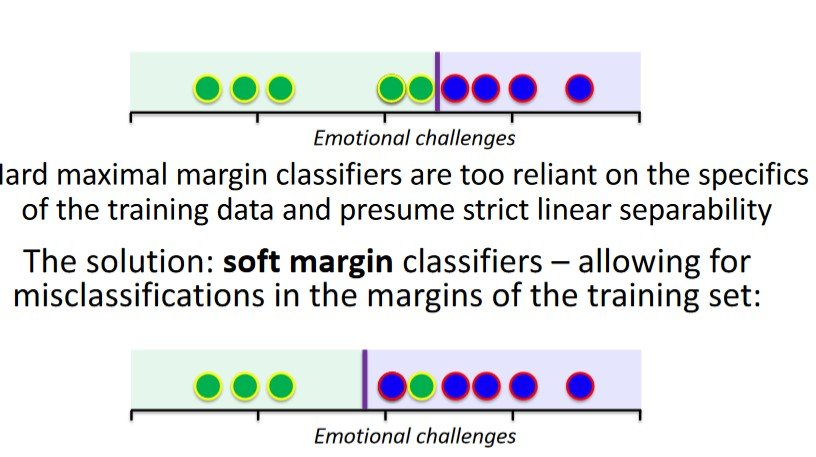
\includegraphics[width=10cm]{Final_Review/lecture_10/hard&soft.jpg}
\item hard margin classifiers are to reliant on the species of the training data 
\item hard marginal classifier require prefect linearly separable data 
\item soft margin classifier allow for some miss classification to make for a more robust classifier overall
\item this is called the bias variance trade off
\subsection{hinge loss }
\item this is a way to penalize the model if it is over fitting to the training data
\item we want to add some penalty term if the distance to the decision boundary is not large enough even if that means making a classification mistake 
\item hinge loss is defined as $L=max(0,1-y_i(w^tx_i+b))$ where $y_i$ is class label so takes on value -1,1 and $(w^tx_i+b)$ is prediction 
\item this introduces some slack into the svm which allows for some more robust classifications
\end{itemize}

\end{document}
